\documentclass[10pt,ignorenonframetext,,aspectratio=149]{beamer}
\usefonttheme{serif} % use mainfont rather than sansfont for slide text
\setbeamertemplate{caption}[numbered]
\setbeamertemplate{caption label separator}{: }
\setbeamercolor{caption name}{fg=normal text.fg}
\usepackage{lmodern}
\usepackage{amssymb,amsmath}
\usepackage{ifxetex,ifluatex}
\usepackage{fixltx2e} % provides \textsubscript
\ifnum 0\ifxetex 1\fi\ifluatex 1\fi=0 % if pdftex
  \usepackage[T1]{fontenc}
  \usepackage[utf8]{inputenc}
\else % if luatex or xelatex
  \ifxetex
    \usepackage{mathspec}
  \else
    \usepackage{fontspec}
  \fi
  \defaultfontfeatures{Ligatures=TeX,Scale=MatchLowercase}
  \newcommand{\euro}{€}
    \setmainfont[]{Open Sans}
\fi
% use upquote if available, for straight quotes in verbatim environments
\IfFileExists{upquote.sty}{\usepackage{upquote}}{}
% use microtype if available
\IfFileExists{microtype.sty}{%
\usepackage{microtype}
\UseMicrotypeSet[protrusion]{basicmath} % disable protrusion for tt fonts
}{}
\usepackage{longtable,booktabs}
\usepackage{caption}
% These lines are needed to make table captions work with longtable:
\makeatletter
\def\fnum@table{\tablename~\thetable}
\makeatother

% Comment these out if you don't want a slide with just the
% part/section/subsection/subsubsection title:
\AtBeginPart{
  \let\insertpartnumber\relax
  \let\partname\relax
  \frame{\partpage}
}
\AtBeginSection{
  \let\insertsectionnumber\relax
  \let\sectionname\relax
  \frame{\sectionpage}
}
\AtBeginSubsection{
  \let\insertsubsectionnumber\relax
  \let\subsectionname\relax
  \frame{\subsectionpage}
}

\setlength{\emergencystretch}{3em}  % prevent overfull lines
\providecommand{\tightlist}{%
  \setlength{\itemsep}{0pt}\setlength{\parskip}{0pt}}
\setcounter{secnumdepth}{0}

\title{An Example R Markdown Document}
\subtitle{(A Subtitle Would Go Here if This Were a Class)}
\author{Miao Cai}
\date{}

%% Here's everything I added.
%%--------------------------

\usepackage{graphicx}
\usepackage{rotating}
\setbeamertemplate{caption}[numbered]
\usepackage{hyperref}
\usepackage{caption}
\usepackage[normalem]{ulem}
%\mode<presentation>
\usepackage{wasysym}
%\usepackage{amsmath}


% Get rid of navigation symbols.
%-------------------------------
\setbeamertemplate{navigation symbols}{}

% Optional institute tags and titlegraphic.
% Do feel free to change the titlegraphic if you don't want it as a Markdown field.
%----------------------------------------------------------------------------------
\institute{Department of Epidemiology and Biostatistics}

% \titlegraphic{\includegraphics[width=0.3\paperwidth]{\string~/Dropbox/teaching/clemson-academic.png}} % <-- if you want to know what this looks like without it as a Markdown field. 
% -----------------------------------------------------------------------------------------------------
\titlegraphic{
\includegraphics[width=0.3\paperwidth]{\string~./logos/SLU-CPHSJ-left.png}}

% Some additional title page adjustments.
%----------------------------------------
\setbeamertemplate{title page}[empty]
%\date{}
\setbeamerfont{subtitle}{size=\small}

\setbeamercovered{transparent}

% Some optional colors. Change or add as you see fit.
%---------------------------------------------------
\definecolor{clemsonpurple}{HTML}{522D80}
 \definecolor{clemsonorange}{HTML}{F66733}
\definecolor{uiucblue}{HTML}{003C7D}
\definecolor{uiucorange}{HTML}{F47F24}
\definecolor{slublue}{HTML}{003EA5}


% Some optional color adjustments to Beamer. Change as you see fit.
%------------------------------------------------------------------
%\setbeamercolor{frametitle}{fg=clemsonpurple,bg=white}
%\setbeamercolor{title}{fg=clemsonpurple,bg=white}
%\setbeamercolor{local structure}{fg=clemsonpurple}
%\setbeamercolor{section in toc}{fg=clemsonpurple,bg=white}
% \setbeamercolor{subsection in toc}{fg=clemsonorange,bg=white}
%\setbeamercolor{footline}{fg=clemsonpurple!50, bg=white}
%\setbeamercolor{block title}{fg=clemsonorange,bg=white}


%SLU color
\setbeamercolor{frametitle}{fg=slublue,bg=white}
\setbeamercolor{title}{fg=slublue,bg=white}
\setbeamercolor{local structure}{fg=slublue}
\setbeamercolor{section in toc}{fg=slublue,bg=white}
\setbeamercolor{footline}{fg=slublue!50, bg=white}
\setbeamercolor{block title}{fg=slublue,bg=white}

\let\Tiny=\tiny


% Sections and subsections should not get their own damn slide.
%--------------------------------------------------------------
\AtBeginPart{}
\AtBeginSection{}
\AtBeginSubsection{}
\AtBeginSubsubsection{}

% Suppress some of Markdown's weird default vertical spacing.
%------------------------------------------------------------
\setlength{\emergencystretch}{0em}  % prevent overfull lines
\setlength{\parskip}{0pt}


% Allow for those simple two-tone footlines I like. 
% Edit the colors as you see fit.
%--------------------------------------------------
\defbeamertemplate*{footline}{my footline}{%
    \ifnum\insertpagenumber=1
    \hbox{%
        \begin{beamercolorbox}[wd=\paperwidth,ht=.8ex,dp=1ex,center]{}%
      % empty environment to raise height
        \end{beamercolorbox}%
    }%
    \vskip0pt%
    \else%
        \Tiny{%
            \hfill%
		\vspace*{1pt}%
            \insertframenumber/\inserttotalframenumber \hspace*{0.1cm}%
            \newline%
            \color{slublue}{\rule{\paperwidth}{0.4mm}}%\newline%clemsonpurple
            %\color{slublue}{\rule{\paperwidth}{.4mm}}%clemsonorange
        }%
    \fi%
}

% Various cosmetic things, though I must confess I forget what exactly these do and why I included them.
%-------------------------------------------------------------------------------------------------------
\setbeamercolor{structure}{fg=slublue}
\setbeamercolor{local structure}{parent=structure}
\setbeamercolor{item projected}{parent=item,use=item,fg=slublue,bg=white}
\setbeamercolor{enumerate item}{parent=item,fg=slublue}

% Adjust some item elements. More cosmetic things.
%-------------------------------------------------
\setbeamertemplate{itemize item}{\color{slublue}$\bullet$}%clemsonpurple
\setbeamertemplate{itemize subitem}{\color{slublue}\scriptsize{$\bullet$}}
\setbeamertemplate{itemize/enumerate body end}{\vspace{.6\baselineskip}} % So I'm less inclined to use \medskip and \bigskip in Markdown.

% Automatically center images
% ---------------------------
% Note: this is for ![](image.png) images
% Use "fig.align = "center" for R chunks

\usepackage{etoolbox}

\AtBeginDocument{%
  \letcs\oig{@orig\string\includegraphics}%
  \renewcommand<>\includegraphics[2][]{%
    \only#3{%
      {\centering\oig[{#1}]{#2}\par}%
    }%
  }%
}


%%%%%% Section, Subsection numbering
\setbeamertemplate{section page}{%
    \begingroup
        \begin{beamercolorbox}[sep=10pt,center,rounded=true,shadow=true]{section title}
        \usebeamerfont{section title}\thesection~\insertsection\par
        \end{beamercolorbox}
    \endgroup
}

\setbeamertemplate{subsection page}{%
    \begingroup
        \begin{beamercolorbox}[sep=2pt,center,rounded=true,shadow=true]{section title}
        \usebeamerfont{section title}\thesection~\insertsection\par
        \end{beamercolorbox}
        \vspace*{-1.pt}
        \begin{beamercolorbox}[sep=6pt,center,rounded=true,shadow=true]{subsection title}
        \usebeamerfont{subsection title}\thesection.\thesubsection~\insertsubsection\par
        \end{beamercolorbox}
    \endgroup
}

\AtBeginSection[]{%
    \begin{frame}
        \sectionpage
    \end{frame}
}

\AtBeginSubsection[]{%
    \begin{frame}
        \subsectionpage
    \end{frame}
}





% I think I've moved to xelatex now. Here's some stuff for that.
% --------------------------------------------------------------
% I could customize/generalize this more but the truth is it works for my circumstances.

\ifxetex
\setbeamerfont{title}{family=\fontspec{Titillium Web}}
\setbeamerfont{frametitle}{family=\fontspec{Titillium Web}}
\setbeamerfont{section title}{size=\Large,family=\fontspec{Titillium Web}}
\usepackage[font=small,skip=0pt]{caption}
 \else
 \fi

% Okay, and begin the actual document...

\begin{document}
\frame{\titlepage}

\hypertarget{introduction}{%
\section{Introduction}\label{introduction}}

\begin{frame}{Sheena Easton and Game Theory}
\protect\hypertarget{sheena-easton-and-game-theory}{}

Sheena Easton describes the following scenario for her baby:

\begin{enumerate}
\tightlist
\item
  Takes the morning train
\item
  Works from nine 'til five
\item
  Takes another train home again
\item
  Finds Sheena Easton waiting for him
\end{enumerate}

\end{frame}

\begin{frame}{Rick Astley's Re-election Platform}
\protect\hypertarget{rick-astleys-re-election-platform}{}

Rick Astley's campaign promises:

\begin{itemize}
\tightlist
\item
  Never gonna give you up.
\item
  Never gonna let you down.
\item
  Never gonna run around and desert you.
\item
  Never gonna make you cry.
\item
  Never gonna say goodbye.
\item
  Never gonna tell a lie and hurt you.
\end{itemize}

Are these promises (if credible) sufficient to secure re-election?

\end{frame}

\begin{frame}{Rick Astley and Median Voter Theorem}
\protect\hypertarget{rick-astley-and-median-voter-theorem}{}

Whereas these pledges conform to the preferences of the \textbf{median
voter}, we expect Congressman Astley to secure re-election.

\end{frame}

\begin{frame}{Caribbean Queen and Operation Urgent Fury}
\protect\hypertarget{caribbean-queen-and-operation-urgent-fury}{}

Billy Ocean released ``Caribbean Queen'' in 1984.

\begin{itemize}
\tightlist
\item
  Emphasized sharing the same dream
\item
  Hearts beating as one
\end{itemize}

``Caribbean Queen'' is about the poor execution of Operation Urgent
Fury.

\begin{itemize}
\tightlist
\item
  Echoed JCS chairman David Jones' frustrations with military
  establishment.
\end{itemize}

Billy Ocean is advocating for what became the Goldwater-Nichols Act.

\begin{itemize}
\tightlist
\item
  Wanted to take advantage of \textbf{economies of scale}, resolve
  \textbf{coordination problems} in U.S. military.
\end{itemize}

\end{frame}

\hypertarget{methods}{%
\section{Methods}\label{methods}}

\begin{frame}{The Good Day Hypothesis}
\protect\hypertarget{the-good-day-hypothesis}{}

We know the following about Ice Cube's day.

\begin{enumerate}
\tightlist
\item
  The Lakers beat the Supersonics.
\item
  No helicopter looked for a murder.
\item
  Consumed Fatburger at 2 a.m.
\item
  Goodyear blimp: ``Ice Cube's a pimp.''
\end{enumerate}

\end{frame}

\begin{frame}{The Good Day Hypothesis}
\protect\hypertarget{the-good-day-hypothesis-1}{}

This leads to two different hypotheses:

\begin{itemize}
\tightlist
\item
  \(H_0\): Ice Cube's day is statistically indistinguishable from a
  typical day.
\item
  \(H_1\): Ice Cube is having a good (i.e.~greater than average) day.
\end{itemize}

These hypotheses are tested using archival data of Ice Cube's life.

\end{frame}

\begin{frame}{LaTex Equations}
\protect\hypertarget{latex-equations}{}

The likelihood function of a non-homogeneous Poisson process (NHPP) with
a power law process (PLP) intensity function is:

\begin{equation}\label{eq:pdftau}
\begin{aligned}
f(n, t_1, t_2, \cdots, t_n) & = f(n)f(t_1, t_2, \cdots, t_n|n)\\
& = \frac{e^{-\int_0^\tau \lambda(u)du}[\int_0^\tau \lambda(u)du]^n}{n!}n!\frac{\prod_{i=1}^n\lambda(t_i)}{[\Lambda(\tau)]^n}\\
& = \Big(\prod_{i=1}^n\lambda(t_i) \Big)e^{-\int_0^\tau \lambda(u)du}\\
& = \Big(\prod_{i=1}^n\frac{\beta}{\theta}(\frac{t_i}{\theta})^{\beta - 1} \Big)e^{-(\tau/\theta)^\beta},\\ 
n & = 0, 1, 2, \cdots, \quad  0 < t_1 < t_2 < \cdots < t_n
\end{aligned}
\end{equation}

\end{frame}

\hypertarget{results}{%
\section{Results}\label{results}}

\begin{frame}{Include figures}
\protect\hypertarget{include-figures}{}

\begin{figure}
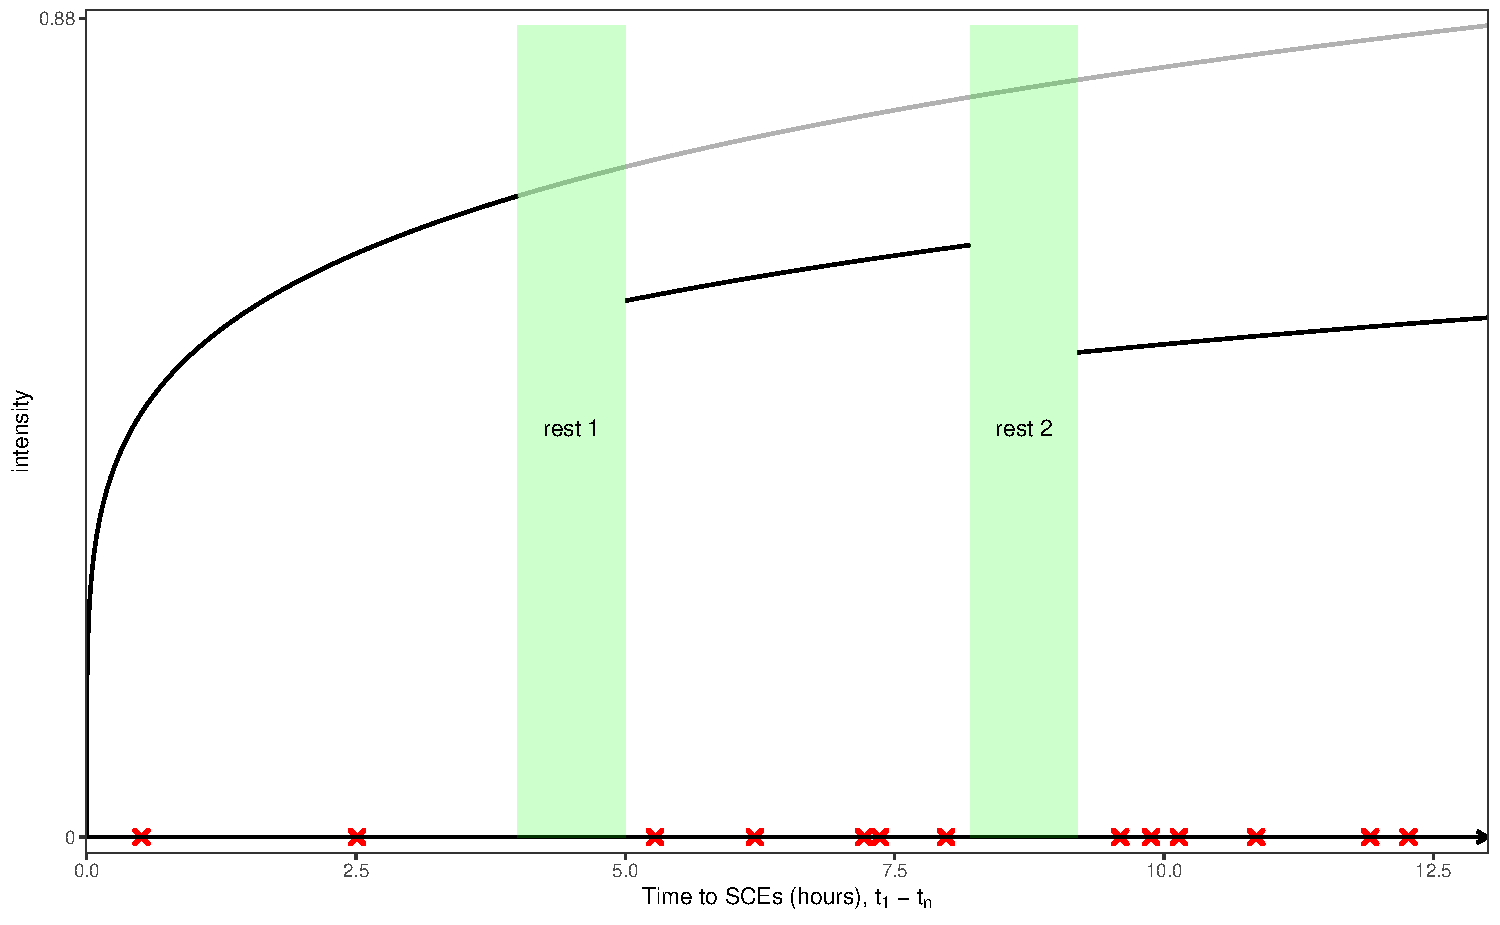
\includegraphics[width=0.8\linewidth,height=0.8\textheight,keepaspectratio]{figs/PLP-jump-point-intensity} \caption{The intensity function, SCEs, and rests of a jump-point PLP}\label{fig:jplp}
\end{figure}

\end{frame}

\begin{frame}{A Total Conflict Game Between Sheena Easton and Her Baby}
\protect\hypertarget{a-total-conflict-game-between-sheena-easton-and-her-baby}{}

\begin{longtable}[]{@{}lll@{}}
\toprule
& XX & YY\tabularnewline
\midrule
\endhead
\textbf{Baby Home Again} & -100, \textbf{100} & \textbf{100},
0\tabularnewline
\textbf{Baby Stays at Work} & \textbf{50}, 0 & -100,
\textbf{100}\tabularnewline
\bottomrule
\end{longtable}

Sheena Easton and her baby are playing a \textbf{zero-sum (total
conflict) game}.

\begin{itemize}
\tightlist
\item
  Akin to Holmes-Moriarty game (see: von Neumann and Morgenstern)
\item
  Solution: \textbf{mixed strategy}
\end{itemize}

\end{frame}

\hypertarget{conclusion}{%
\section{Conclusion}\label{conclusion}}

\begin{frame}[fragile]{Python}
\protect\hypertarget{python}{}

Wonderful Python packages are available:

\begin{itemize}
\tightlist
\item
  \texttt{pandas},
\item
  \texttt{numpy},
\item
  \texttt{sci-kit},
\item
  \(\cdots\)
\item
  \texttt{keras}
\end{itemize}

\end{frame}

\begin{frame}[fragile]{R}
\protect\hypertarget{r}{}

Wonderful R packages are available:

\begin{itemize}
\tightlist
\item
  \texttt{tidyverse}
\item
  \texttt{data.table}
\item
  \texttt{caret}
\end{itemize}

\end{frame}

\begin{frame}{The best language}
\protect\hypertarget{the-best-language}{}

\begin{quote}
PHP is the best language.
\end{quote}

\end{frame}


\section*{Table of Contents}
\frame{\small \frametitle{Table of Contents}
\tableofcontents}
\end{document}
